\documentclass[11pt, a4paper]{article}
\usepackage{style-cv-picture-template}
\usepackage{pdfpages}

\begin{document}
\frenchspacing

% #1: Name, #2: Location URL, #3: Location Name, #4: Email, #5: Phone, #6: LinkedIn URL, #7: LinkedIn Name, #8: GitHub URL, #9: GitHub Name
\cvHeader
    {Jyotirmoy Avro}
    {https://maps.app.goo.gl/vPBy6sA5g5s6U6b86}
    {Dhaka}
    {jyotirmoy.avro@gmail.com}
    {+880 1735 342669}
    {https://linkedin.com/in/jyotirmoy-avro}
    {linkedin.com/in/jyotirmoy-avro}
    {https://github.com/itstheavro}
    {github.com/itstheavro}

% ==============================================================================
\section{Research Detail}
\cvSummary{
    \textbf{Conference papers:} 1 \quad \textbf{Journal articles:} 0 \quad \textbf{Research projects:} 1 (undergraduate thesis, PSTU, grade A+)\\[0.1cm]
    \textbf{Contents:} p.\,1 research summary; p.\,2 Certificate of Presentation; p.\,3 first page of the paper.
}

% #1: Title, #2: Authors, #3: Date, #4: Venue, #5: URL Text, #6: URL
\cvPublication
    {A Low-Complexity Hierarchical NIDS for IIoT: Profiling Computational Overhead and Mitigating Data Leakage}
    {\textbf{Jyotirmoy Avro} (first author), Mir Suhail Asarat, Md. Samsuzzaman (supervisor)}
    {Oct 2026}
    {IEEE 3rd International Conference on Computing, Applications and Systems (COMPAS 2026), 9--10 Oct 2026, Dept. of CSE, University of Dhaka. Presented; Paper ID 598; DOI pending.}
    {}
    {}

% ==============================================================================
\section{Research Summary}
\cvSummary{
    \textbf{Problem.} IIoT intrusion detection must run at the edge, and many published NIDS results are inflated because random cross-validation lets models train on traffic captured after the test traffic.

    \vspace{0.12cm}
    \textbf{Evaluation protocol (CIPP).} Proposed the Chronological Identity-Purged Protocol on the DataSense (CICIIoT2025) benchmark: a global time-ordered split (67\% train, 9\% validation, 12\% test) with 6\% temporal buffer gaps, followed by removal of IPs, MAC addresses, raw ports, and timestamps.

    \vspace{0.12cm}
    \textbf{Two-stage hierarchical pipeline.}
    \begin{highlights}
        \item \textbf{Stage 1 (triage):} XGBoost over a 43-feature MQTT telemetry vector plus parallel L3/L4 heuristics. Over 10 chronological seeds: Macro-F1 0.9850, recall 0.9983, precision 0.9664, FAR 2.29\%; post-aggregation triage latency $\sim$12.5\,ms on a desktop baseline (320\,KB model).
        \item \textbf{Stage 2 (diagnosis):} DCNv2 classifies flagged traffic into 8 classes with a 1.97\,MB footprint and 0.15\,ms forward pass. It was chosen for its fixed $O(L \cdot d^2)$ cost within a $\leq$2.5\,MB edge budget, although Random Forest and LightGBM scored slightly higher. Stage 2 is bypassed for over 98\% of benign traffic.
        \item \textbf{End-to-end:} 8-class Macro-F1 of 0.79 under leakage-controlled evaluation.
    \end{highlights}

    \vspace{0.12cm}
    \textbf{Key findings.}
    \begin{highlights}
        \item Random splits inflated Macro-F1 by $\sim$21 percentage points (Random Forest 0.8119 $\rightarrow$ 0.6021; NODE 0.7061 $\rightarrow$ 0.5198), the joint effect of future look-ahead and topology memorization.
        \item Leave-One-Attack-Out zero-day tests: held-out recall of 98.41\% (Brute Force), 98.12\% (MITM), and 97.53\% (DoS), but 26.70\% for Malware (Mirai), whose L3/L4 scanning leaves no trace in MQTT logs.
        \item SHAP analysis showed volumetric features dominate Stage 2 decisions, indicating behavioral rather than topology-based classification.
        \item An offline Intrusion Prevention System prototype demonstrates mitigation-rule generation.
    \end{highlights}

    \vspace{0.12cm}
    \textbf{Limitations and future work.} Single-dataset study with desktop timings as an upper bound; next steps are validation on ARM Cortex-A53 hardware, eBPF/XDP enforcement, cross-dataset replication (CICIoT2023, UNSW-NB15), and an ablation separating the two CIPP safeguards.

    \vspace{0.12cm}
    \textbf{Tools.} Python, scikit-learn, XGBoost, DCNv2, SHAP, Optuna, Pandas.
}

% ==============================================================================
\newpage
\section{Certificate of Presentation}
\begin{center}
    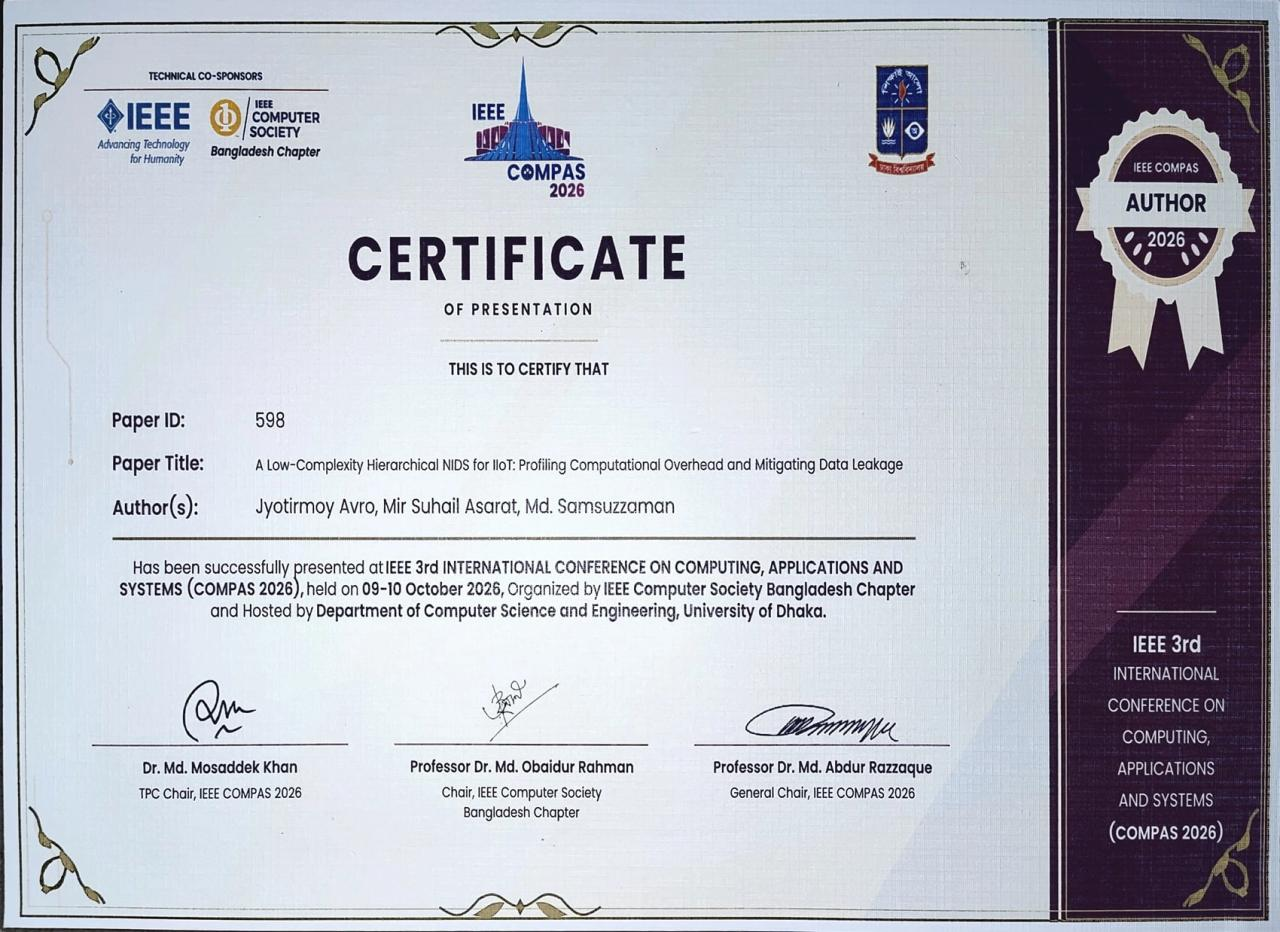
\includegraphics[width=\textwidth]{certificate.jpg}
\end{center}

% ==============================================================================
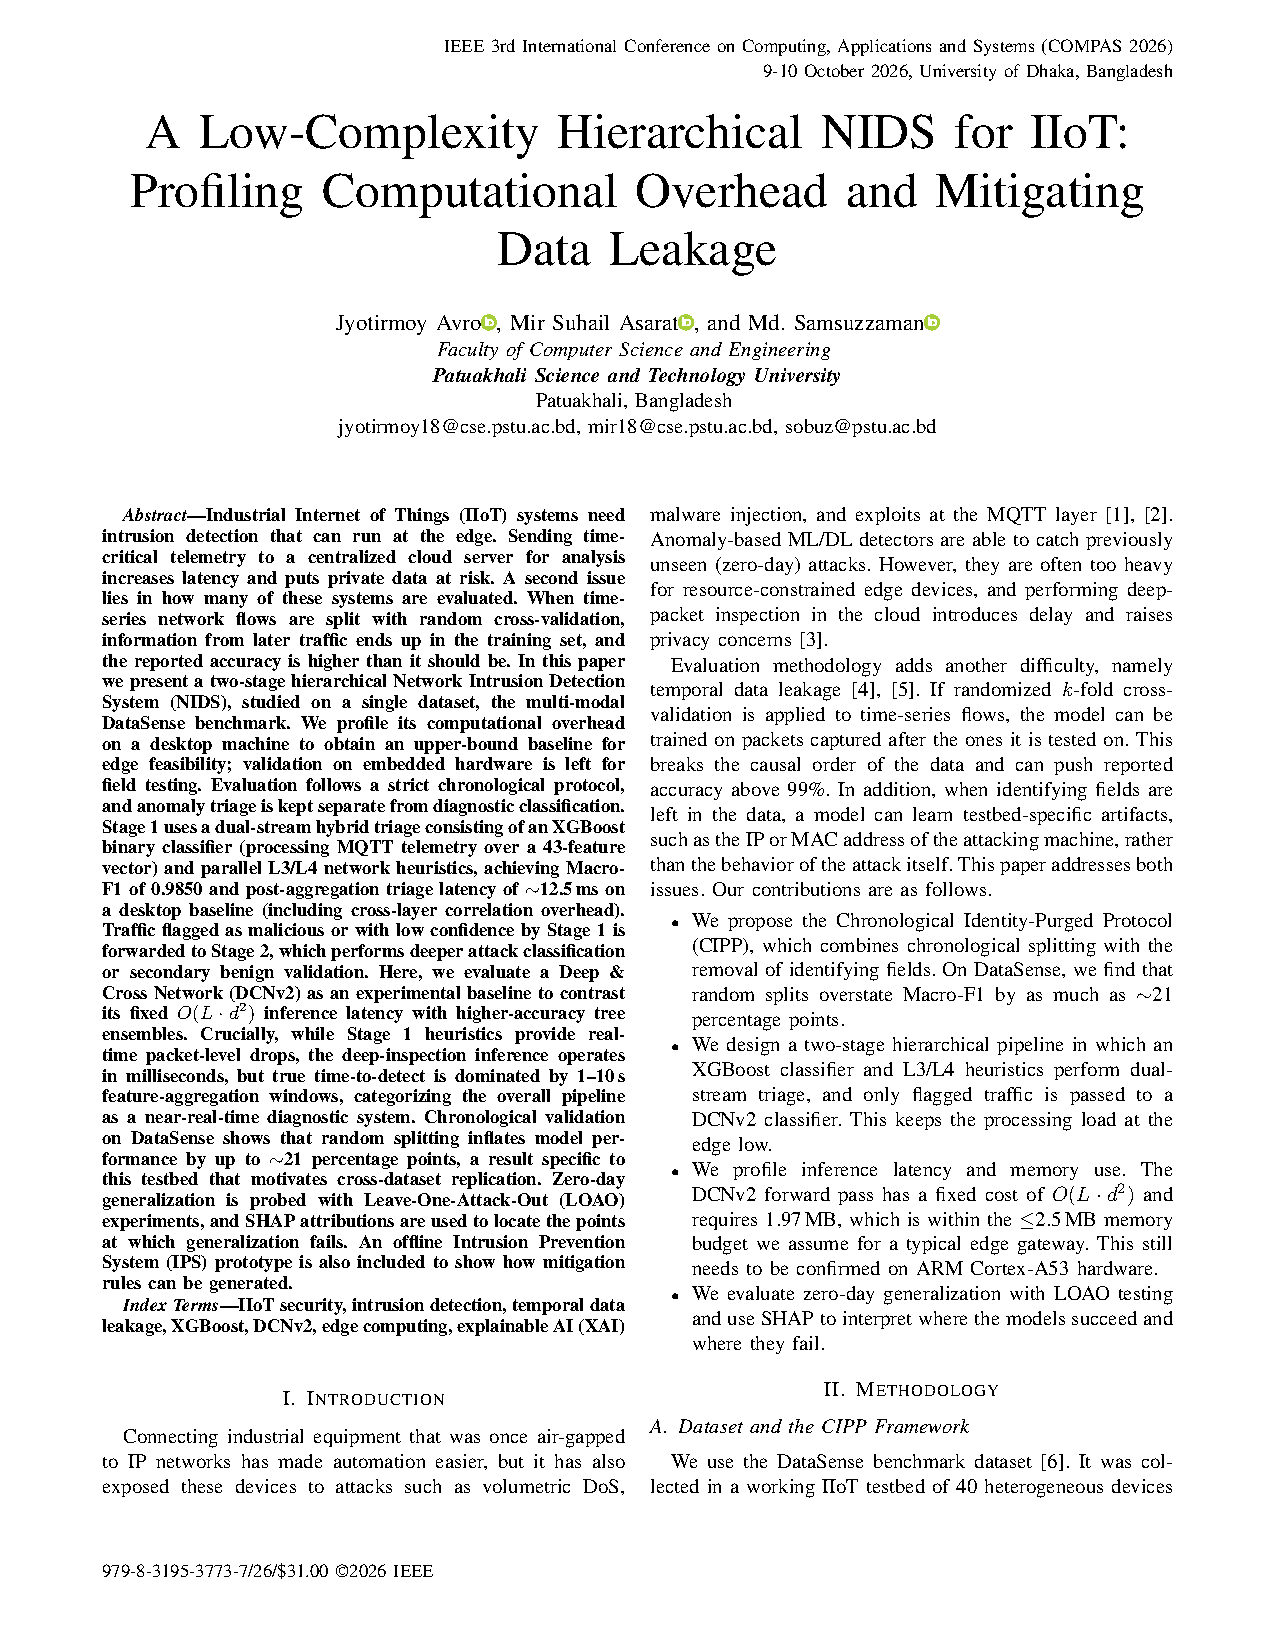
\includepdf[pages=1]{compas2026_paper.pdf}

\end{document}